% Template for Carleton student papers
% Author: Andrew Gainer-Dewar, 2013
% This work is licensed under the Creative Commons Attribution 4.0 International License.
% To view a copy of this license, visit http://creativecommons.org/licenses/by/4.0/ or send a letter to Creative Commons, 444 Castro Street, Suite 900, Mountain View, California, 94041, USA.
\documentclass[12pt,twoside,leqno,fleqn,letterpaper]{article}
\usepackage[style=apa, backend=biber, natbib=true, language=american]{biblatex}
\usepackage[T1]{fontenc}
\usepackage{nicematrix}
\usepackage{ragged2e}
\DeclareLanguageMapping{american}{american-apa}
% \renewcommand*{\nameyeardelim}{\addcomma\space}
\renewcommand*{\postnotedelim}{\addsemicolon\space}

\newrobustcmd*{\postcite}[1]{%
  \nocite{#1}\entrydata{#1}{\usebibmacro{cite}}
  }
\newrobustcmd*{\postcitemult}[2]{%
\nocite{#1}\entrydata{#1}{\usebibmacro{cite}},
\nocite{#2}\entrydata{#2}{\usebibmacro{cite}}
}
\usepackage{nicematrix}

% % APA-specific adjustments
% \AtBeginBibliography{\renewcommand*{\mkbibnamefamily}[1]{\textsc{#1}}} % APA-style author capitalization in bibliography

% % Other biblatex adjustments to mimic APA style
% \DeclareNameAlias{sortname}{last-first} % Last name, first name format
% \DeclareNameAlias{default}{last-first}

\addbibresource{sources.bib}
% % Add a comma between author and year for in-text citations
% \renewcommand{\nameyeardelim}{\addcomma\space}
% \newcommand{\texteq}[2][0.5]{\text{\parbox[t]{#1\displaywidth}{#2}}}
% \newcommand{\lther}{\mathord{\therefore}\mskip\thickmuskip}
%-----------------------------------------------------------------
% Lengths to control indents of 'equation numbers' and statements
\newlength{\numbersep}          % Distance of number at left margin
\newlength{\statementsep}       % Distance of statement at left margin
\setlength{\numbersep}{\parindent}  % n
\setlength{\statementsep}{15mm}    % m (0<n<m) 
%-----------------------------------------------------------------
\everydisplay{\displayindent=\numbersep}
\setlength{\mathindent}{\statementsep}
% \setlength{\mathindent}{3cm}
\usepackage{ccpaper}
\usepackage{setspace, graphicx, caption} %\doublespacing
\usepackage{geometry, tikz, nccmath, graphbox}
\usepackage{tikzsymbols}
\usepackage{gensymb,algorithm2e}
\RestyleAlgo{ruled}
\allowdisplaybreaks
\geometry{portrait, margin=1in}
\usepackage[title]{appendix}
\usetikzlibrary{shapes.geometric}
\usetikzlibrary{arrows.meta,arrows}
\usetikzlibrary{positioning}
% \usepackage{cite}
% The Latin Modern font is a modernized replacement for the classic
% Computer Modern. Feel free to replace this with a different font package.
\usepackage{lmodern}
\usepackage{preamble2}
\newcommand{\Bias}[2]{\text{Bias}_{\text{#2}} \left(#1\right)}


% \makeatletter
% \newcommand{\myitem}[1]{%
% \item[#1]\protected@edef\@currentlabel{#1}%
% }
% \makeatother

% Define a new item command with custom labels and references
\newlist{myenumerate}{enumerate}{1}
\setlist[myenumerate,1]{
    label={\theenumi.},     % Labels will include dots (e.g., P1., C1., etc.)
    ref={\theenumi},
    leftmargin=*,       % Indent matches paragraph indentation
    labelindent=1.6\parindent
    % ,
    % widest=P8,              % Adjusts width to align with the widest label (optional)
}

% Customize counters for P and C items
\makeatletter
\newcommand{\myitem}[1]{%
    \item[\textbf{#1.}]%
    \def\@currentlabel{#1}% Set the label for referencing
}
\makeatother

\makeatletter
\newcommand{\myitemA}[1]{%
    \item[$\mathbf{#1:}$]%
    \def\@currentlabel{$\mathbf{#1}$}% Set the label for referencing
}
\makeatother

\makeatletter
\newcommand{\myitemB}[1]{%
    \item[$#1:$]%
    \def\@currentlabel{$\#1$}% Set the label for referencing
}
\makeatother

% Load in biblatex
% To use a different bibliography style, just change "numeric" to
% your pautoreferred style (mla for MLA style, alphabetic for Author-Year
% style, etc.) There are a lot of options; check the BibLaTeX documentation.
% \usepackage{natbib}

% Select the bibliography file
\usepackage{csquotes}
\usepackage{coffee4}
%Use single spacing, set 10pt font, set italics, and beginning quotes
% \renewcommand{\mkbegdispquote}
%     {\selectfont\textooquote}%\setquotestyle{quote}
% %End displayquote environment with ending quotes
% \renewcommand{\mkenddispquote}{\textcoquote}

\title{\textbf{LA Nurse BP}}
\subtitle{Case Study 1\footnote{Code used for this project is available at this \href{https://github.com/kwlyu/stat330-w25-case-study-1.git}{GitHub Repository}.}} %Optional. Omit if not wanted.
\author{Kunwu Lyu}
\date{Feburary 13, 2025}

\prof{Katie St. Clair}
\course{STAT 330}
\usepackage{epigraph}
\setlength\epigraphwidth{.8\textwidth}
\setlength\epigraphrule{0pt}
\renewcommand*{\bibfont}{\normalfont \small}
% \usepackage{etoolbox}
% \apptocmd{\thebibliography}{\interlinepenalty 1000000\relax}{}{}
% To enable double spacing, uncomment this line:
\titlespacing*{\section}
{0pt}{0ex}{0ex}
\titlespacing*{\subsection}
{0pt}{0ex}{0ex}
\usepackage{sectsty}
\sectionfont{\fontsize{12}{12}\selectfont}
\subsectionfont{\fontsize{12}{12}\selectfont}

\theoremstyle{definition}
\newtheorem{theorem}{Theorem}[section]
\newtheorem{corollary}{Corollary}[theorem]
\newtheorem{lemma}{Lemma}[theorem]
\theoremstyle{definition}
\newtheorem{definition}{Definition}[section]
\usepackage{xpatch}
\xpatchcmd{\NCC@ignorepar}{%
\abovedisplayskip\abovedisplayshortskip}
{%
\abovedisplayskip\abovedisplayshortskip%
\belowdisplayskip\belowdisplayshortskip}
{}{}

\usepackage{verbatim}
\newcommand{\detailtexcount}[1]{ %
\immediate\write18{texcount -merge -sum #1.tex > #1.wcdetail }%
\verbatiminput{#1.wcdetail}%
}

% \usepackage{verbatim}

% \newcommand{\detailtexcount}[1]{%
%   \immediate\write18{texcount -merge -sum -q #1. > #1.wcdetail }%
%   \verbatiminput{#1.wcdetail}%
% }
% Reduce space before and after the array environment
\setlength{\abovedisplayskip}{0pt}
\setlength{\belowdisplayskip}{0pt}
% \setcounter{section}{-1}
% Reduce space in enumerate environment
\setlist{nosep}
\begin{document}
\renewcommand{\abstractname}{Executive Summary}
\maketitle{\vspace{-6ex}}
\setlength{\parskip}{0.2cm}
\setlength{\mathindent}{31pt}
\expandafter\def\expandafter\normalsize\expandafter{%
    \normalsize%
    \setlength\abovedisplayskip{0pt}%
    \setlength\belowdisplayskip{0pt}%
    \setlength\abovedisplayshortskip{0pt}%
    \setlength\belowdisplayshortskip{0pt}%
}
% \cofeAm{0.4}{0.8}{0}{5.5cm}{9cm}
% \doublespacing
\singlespacing

\begin{abstract}
    Here is what I did.
\end{abstract}

\section{Introduction}

Certain traits such as family history and mood are expected to increase one's ambulatory blood pressure (BP). \citet{goldstein_ambulatory_2000} studied potential factors that contribute to hypertension. They collected information about the participants' BP, activity levels, work status, and mood ratings throughout the day, as well as relevant family history and information about their menstrual phases, to establish links that lead to elevated BP. Towards the end, they sought to uncover preventative measures for individuals who may be at a higher risks of developing hypertension. The objectives of this project is much simpler. I am interested in exactly what traits are \emph{associated} with elevating one's BP, given the longitudinal structure and various time-dependent metrics in the dataset \parencites(given by)()[cited by \postcite{roback_beyond_2021}]{goldstein_ambulatory_2000}.

\subsection{Methods}

The dataset includes repeated measures over the course of two work and off-work days on 203 registered nurses between the ages of 24 and 50 years working in Los Angeles, in the year 2000. Of those 203 nurses, 172 has complete data on all of the variables recorded.\footnote{In the original paper by Goldstein and Shapiro \pnotecite[228-29]{goldstein_ambulatory_2000}, they reported 171 nurses who completed all sessions. It is likely that this is due to \citet{roback_beyond_2021} or \citet{weiss_modeling_2005} excluding other personality variables used in the original study. Because I am not investigating personality traits in this project, 172 suffices being my total subject counts. Additionally, Goldstein and Shapiro  mention that ``[s]imilar patterns of findings were obtained in the sample of 171 as in the total sample'' \pnotecite[229]{goldstein_ambulatory_2000}.} BP of the participants were measured 30 minutes before their normal start of work, and measured measured repeatedly every 20 minutes for the rest of the day. This led to around 40-60 observations per nurse (9573 total observations). Each time the BP was taken, participants were asked to give several mood ratings including happiness, stress, and tiredness. In addition, participants wore an actigraph on their waist to record frequency of movements in one-minute intervals; the researchers obtained an activity measure for the ten-minute periods before each BP reading.

\section{Exploratory Data Analysis}

The variables (original and re-parameterized) used in this project are given in \Cref{tab: var desc}. Variable missingness was explored in \Cref{fig: missing}. We see that the data were missing primarily mood ratings and some activity levels from several participants. Because I am interested in how both of these variables relate to BP, I will proceed the analysis with the missing rows removed, leaving us with a total of 172 participants and 7877 observations. The visuals and statistics below will be given in terms of that subset of the data, unless otherwise specified.

\begin{table}[H]
    \centering\begin{tabular}{|p{0.2\linewidth} | p{0.65\linewidth}|}
        \hline
        Variable Name & Variable Descrption \\
        \hline\hline
        ID (Cluster) & Unique identification number for each participant \\
        \hline
        BP (Response) & Systolic blood pressure (in mmHg) \\
        \hline
        \textcolor[RGB]{208, 2, 27}{Act} & Activity level (frequency of movements in 1-minute intervals, over a 10-minute period) \\
        \hline
        \textcolor[RGB]{74, 144, 226}{Phase} & Menstrual phase (follicular or luteal) \\
        \hline
        \textcolor[RGB]{74, 144, 226}{Day} & Workday or non-workday \\
        \hline
        \textcolor[RGB]{208, 2, 27}{Posture} & Position during BP measurement (sitting, standing, or reclining) \\
        \hline
        \textcolor[RGB]{208, 2, 27}{HAP} & Self-ratings of happiness by each nurse at the time of each BP measurement on a 5-point scale (5 strongest and 1 weakest) \\
        \hline
        \textcolor[RGB]{208, 2, 27}{STR} & Self-ratings of stress by each nurse at the time of each BP measurement on a 5-point scale (5 strongest and 1 weakest) \\
        \hline
        \textcolor[RGB]{208, 2, 27}{TIR} & Self-ratings of tiredness by each nurse at the time of each BP measurement on a 5-point scale (5 strongest and 1 weakest) \\
        \hline
        \textcolor[RGB]{74, 144, 226}{Age} & Age (in years) \\
        \hline
        \textcolor[RGB]{74, 144, 226}{Full FH} & Family history, coded as either NO (no family history of  hypertension), YES (1 hypertensive parent), or YESYES (both parents hypertensive) \\
        \hline\hline
        \emph{\textcolor[RGB]{208, 2, 27}{Stand}} & Indicator variable for standing, where it equals 0 if Posture is either sitting or reclining and 1 when Posture is standing \\
        \hline
        \emph{\textcolor[RGB]{208, 2, 27}{Mood}} & Combined mood ratings: HAP - (STR + TIR)/2 \\
        \hline
        \emph{\textcolor[RGB]{74, 144, 226}{FH}} & Indicator variable for having family history of hypertension (1 for YES and YESYES, 0 for NO) \\
        \hline
        \emph{\textcolor[RGB]{74, 144, 226}{Age24}} & Recentered Age: Age - 24 \\
        \hline
        \multicolumn{2}{c}{\footnotesize Note: \emph{emphasis} added to re-parameterized variables; colors represent levels.}
    \end{tabular}
    \caption{Variable Descrptions}
    \label{tab: var desc}
\end{table}

\begin{figure}
\centering
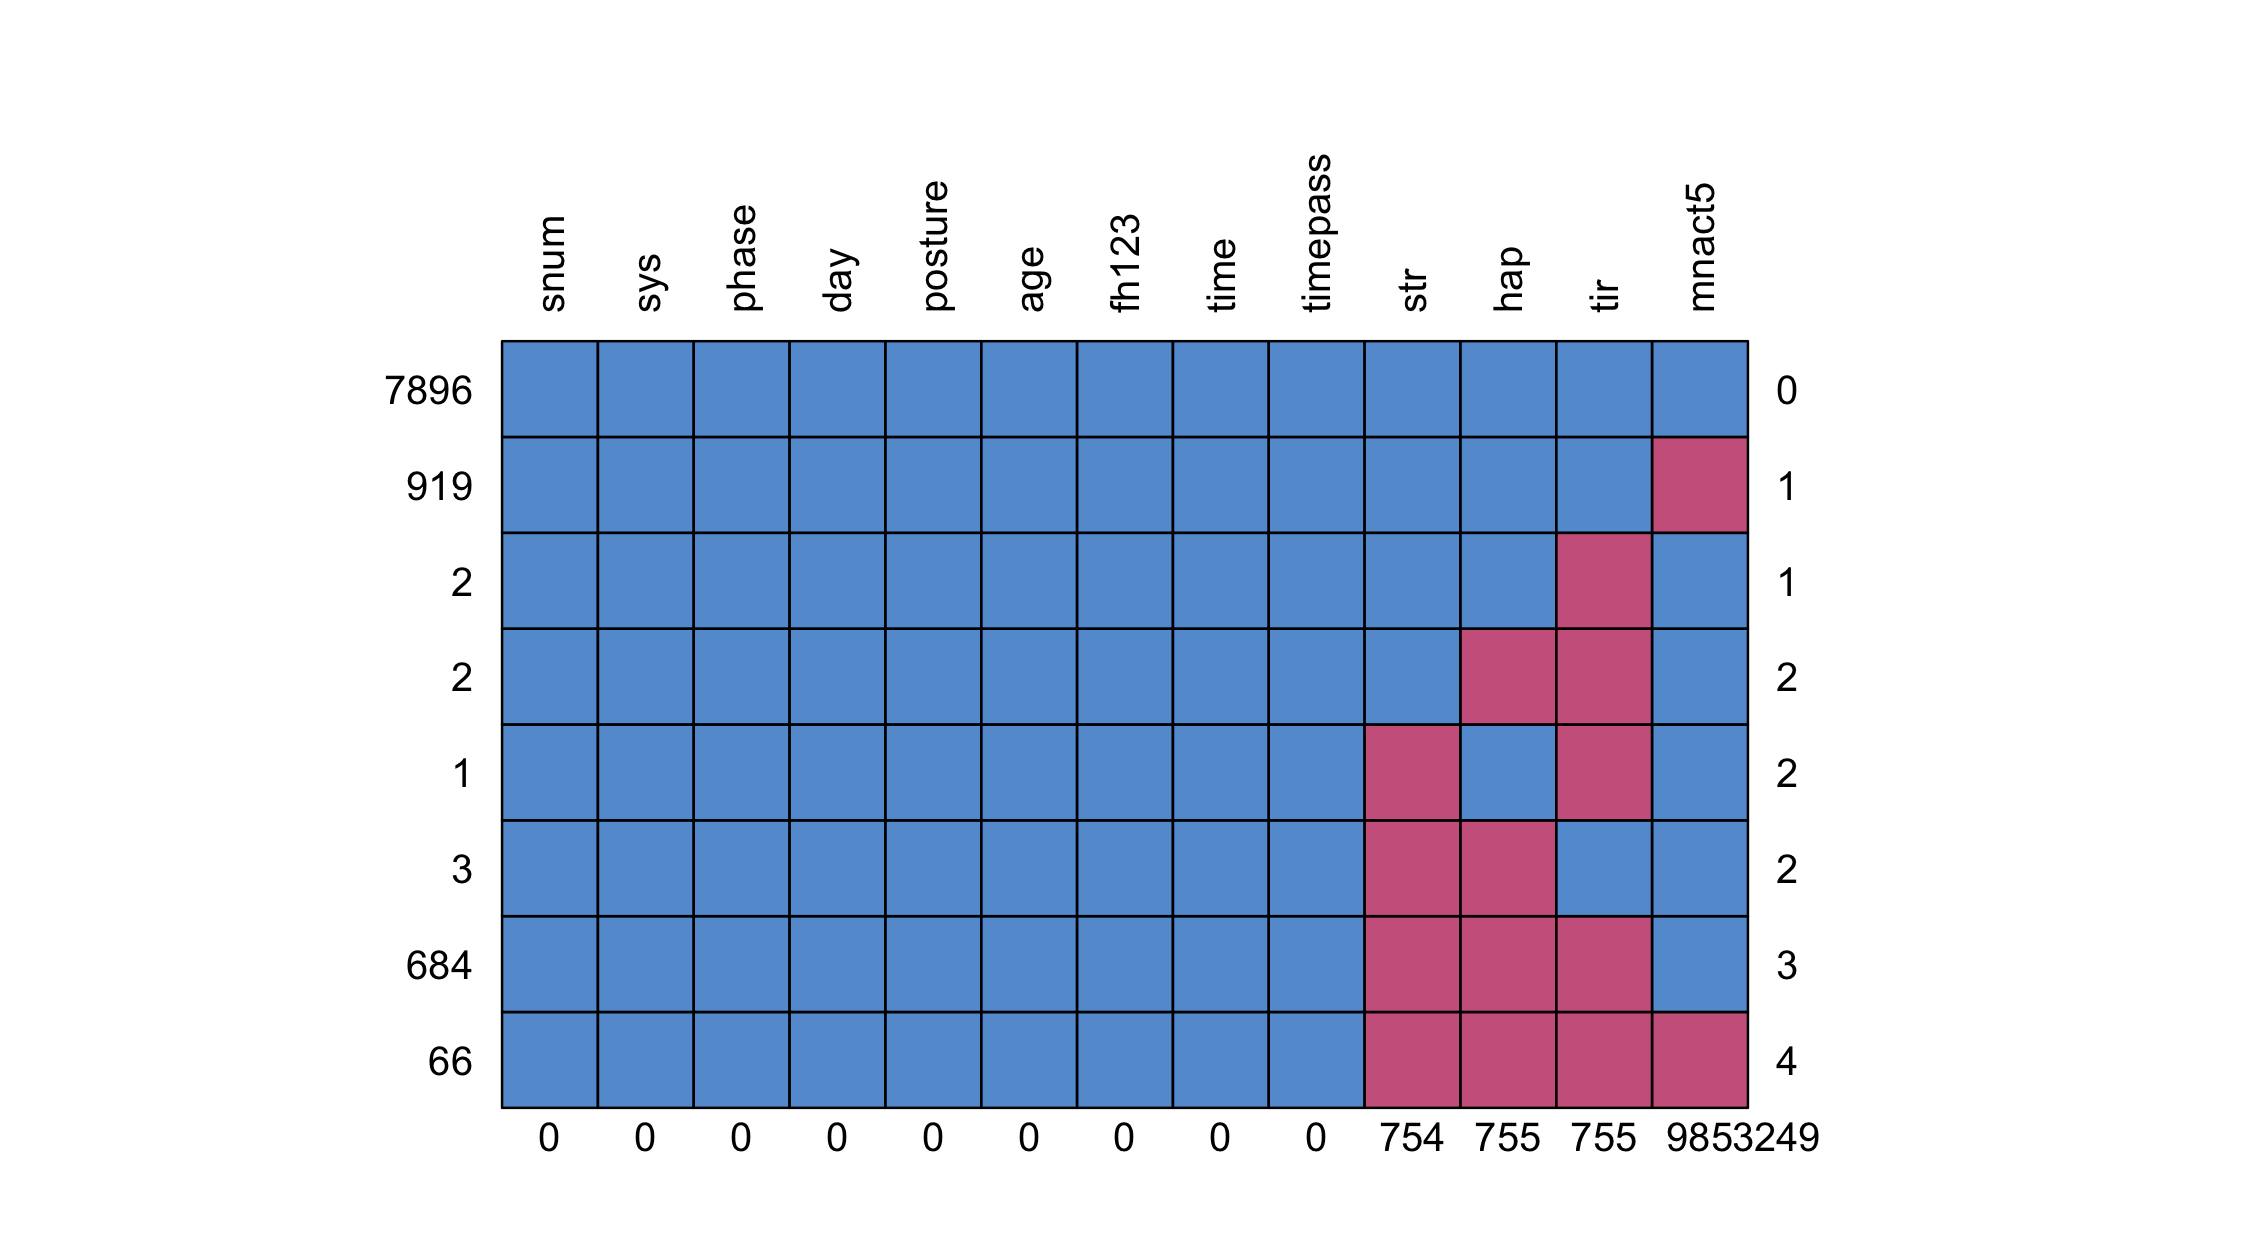
\includegraphics[width=\textwidth]{pics/miss.png}
\caption{Data Missingness}
\label{fig: missing}
\end{figure}

Because of the longitudinal nature of our data, it is worth noting our levels of analysis and to which our variables belong. I will call time-dependent measurements \emph{\textcolor[RGB]{208, 2, 27}{Level 1}} data (variables) and the rest of the subject-level measurements \emph{\textcolor[RGB]{74, 144, 226}{Level 2}} data (variables). Each participant has a unique identification number; this will distinguish between different clusters. Our primary response is systolic blood pressure (BP), and I will use our exploratory data analysis below to guide our model selection process from the bottom-up.

Note that I created three additional variables from the original dataset to help simplify the modeling process. In the original dataset, \texttt{Posture} is a factor variable with three levels: Recline ($n = 530$), Sit ($n = 3644$), and Stand ($n = 3703$). Because the relatively small number of observations where participants were reclining (presumably sleeping at night or resting), I collapsed the three levels into either Standing or non-Standing. Similarly, because of the relatively small number of participants have both parents with hypertension ($n = 13$), I collapsed it together with having one parent with hypertension ($n = 66$) to compare against those without any family history ($n = 103$). Lastly, a general \texttt{Mood} measurement was created by subtracting the average of tiredness and stress from happiness. 

\subsection{Level 1 by Clusters}

I will first explore how BP vary among participants and how it relates to the level 1 predictors to examine if there is any sign of clustering between different participants (which is the premise of a longitudinal study). From \Cref{fig: bp by subjects}, we see that BP readings do tend to vary among different participants, though variations within each participant do not seem to be pronounced. This suggests that a Linear Mixed Model (LMM) might be more appropriate than a regular Multiple Linear Regression (MLR).

Since our data is ordered in time, one might be interested in answering how the participants' BP evolve over time. For sake of brevity, I show a random subsets of subjects and their BP readings over time in \Cref{fig: bp v time facet}. From this plot alone, not much could be deciphered; some trends (e.g., participant 1116) seem to decrease over time while others either slightly increase (e.g., participant 1267) or do not see much fluctuation overall. Indeed, when I fit separate linear smoothers for each participant, I see various different intercepts and slopes for each participant (see \Cref{fig: bp v time separate ls}). This suggests that a random effect for both the intercept and slope of time.

\begin{figure}
\centering
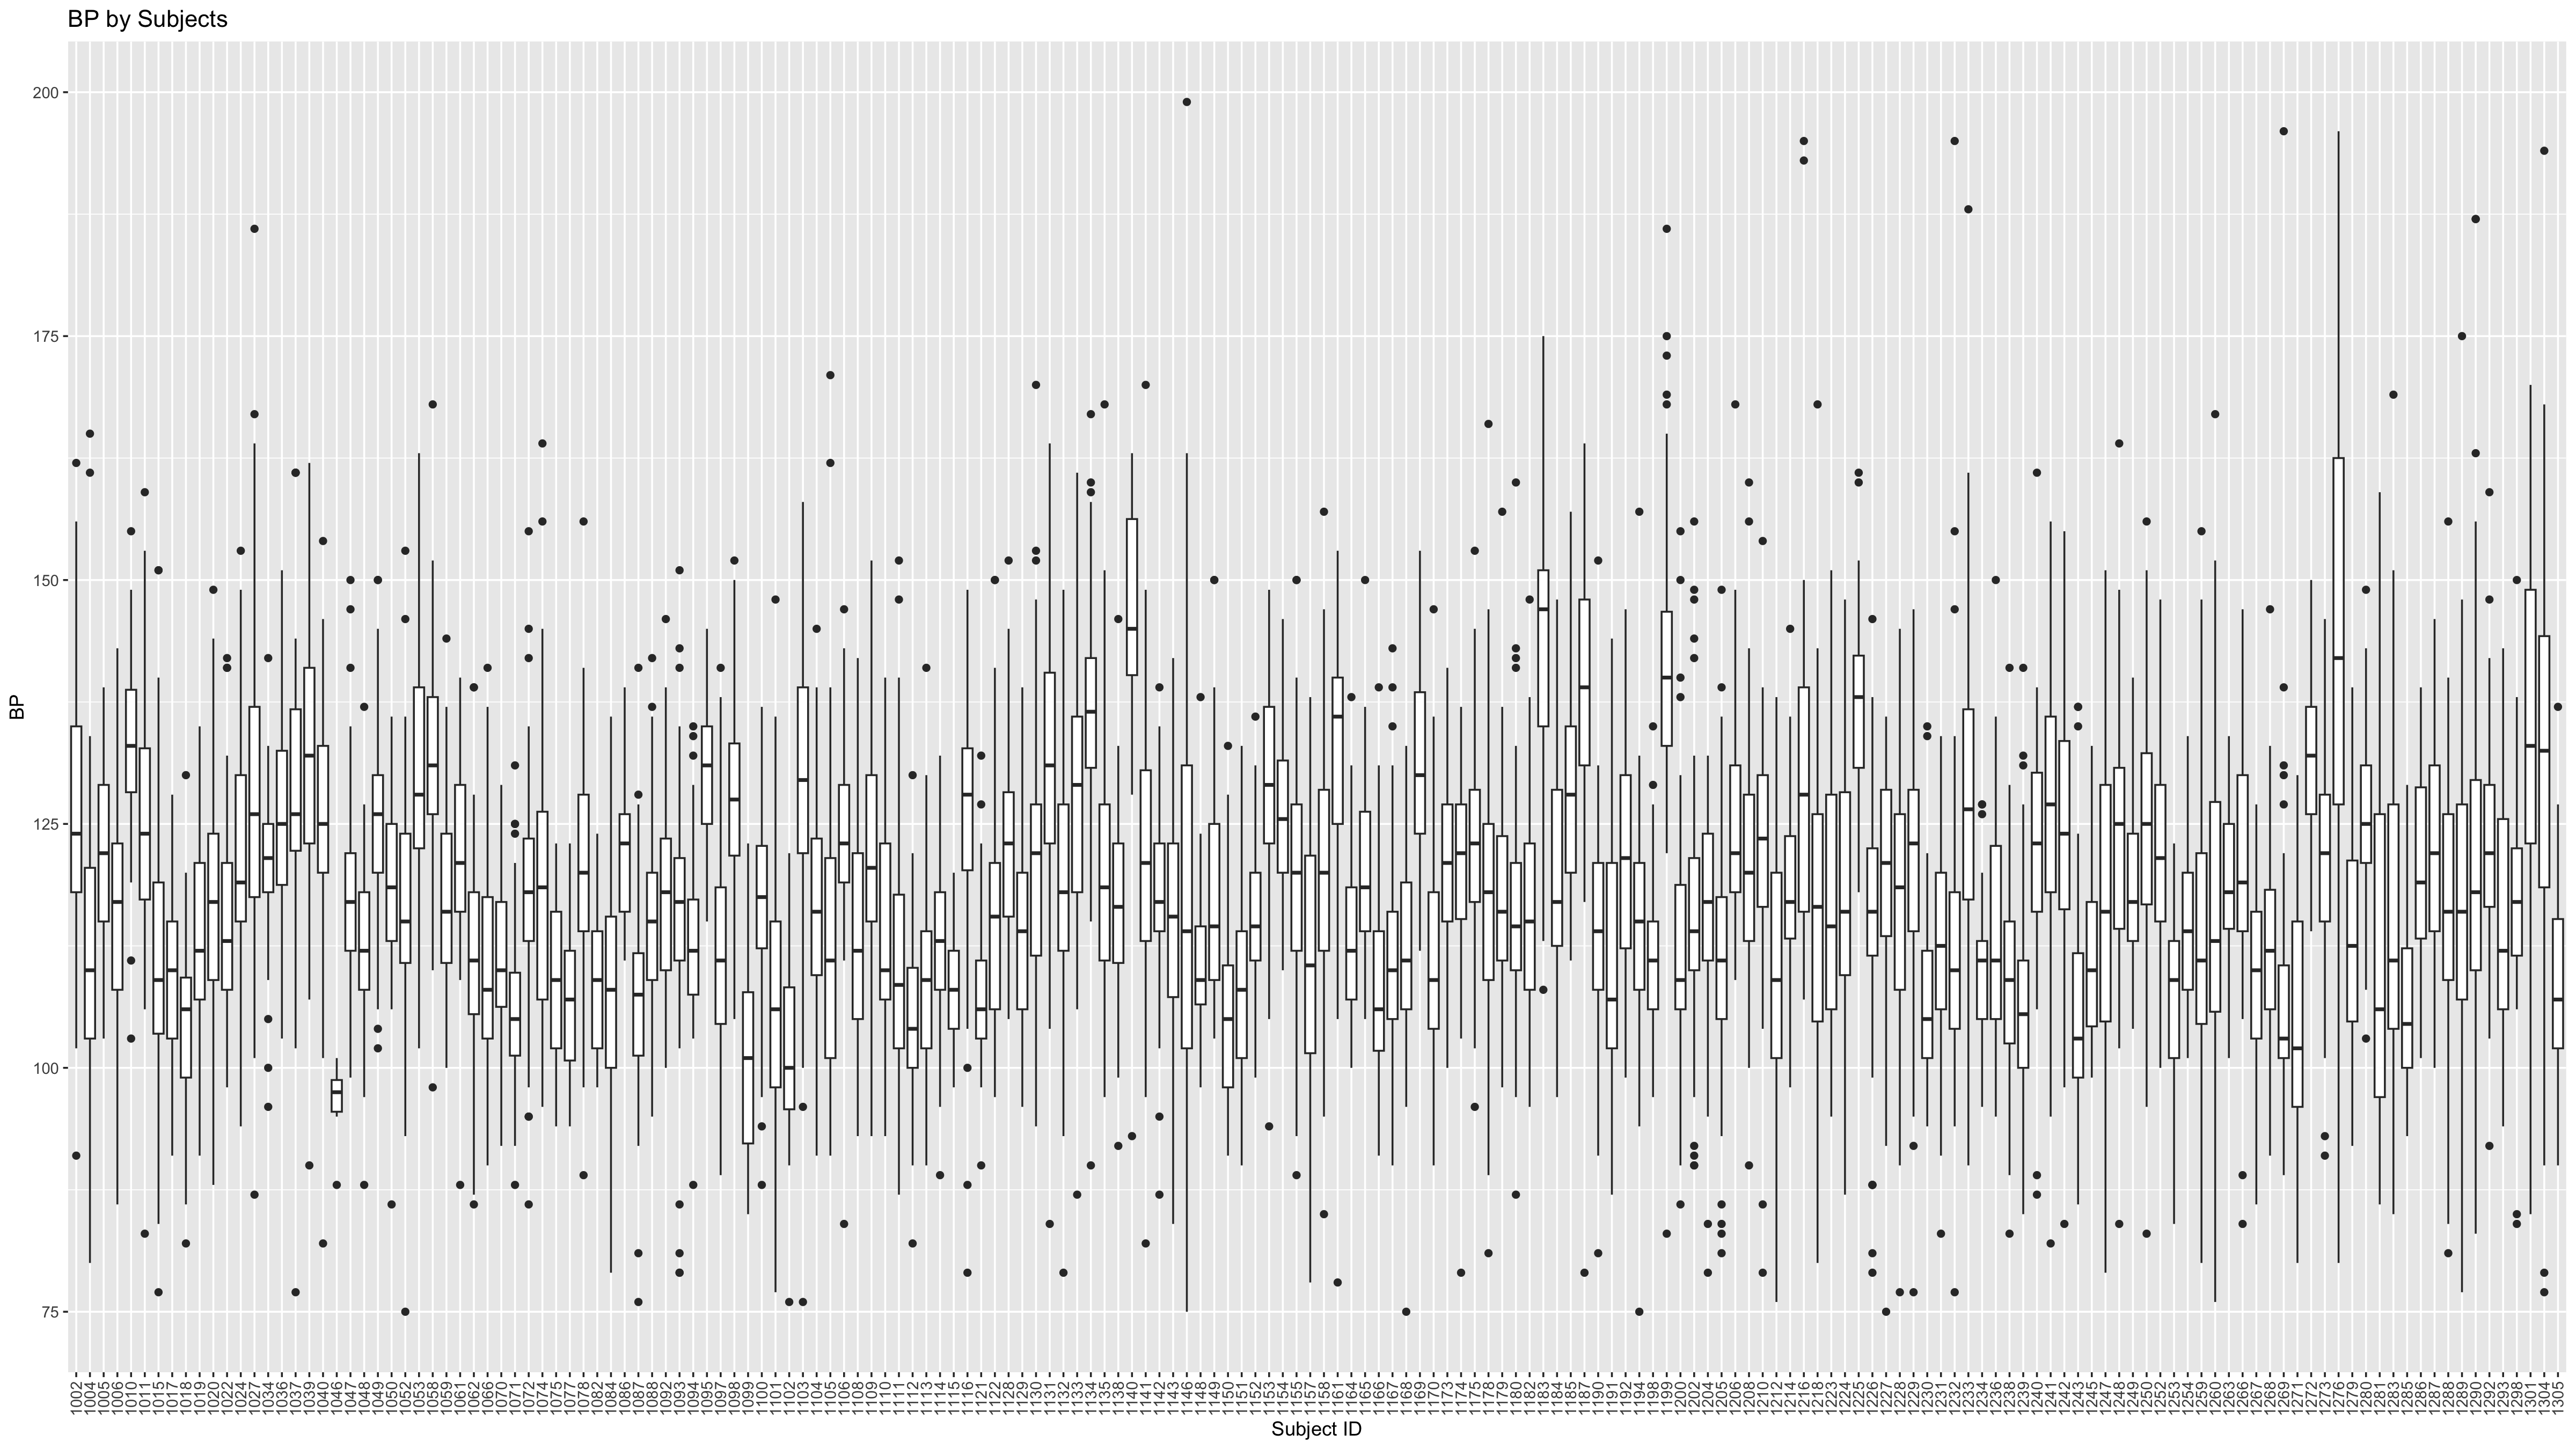
\includegraphics[width=\textwidth]{pics/bp by subjects.png}
\caption{BP by Subjects}
\label{fig: bp by subjects}
\end{figure}

\begin{figure}
\centering
\begin{subfigure}[b]{0.475\textwidth}
\centering
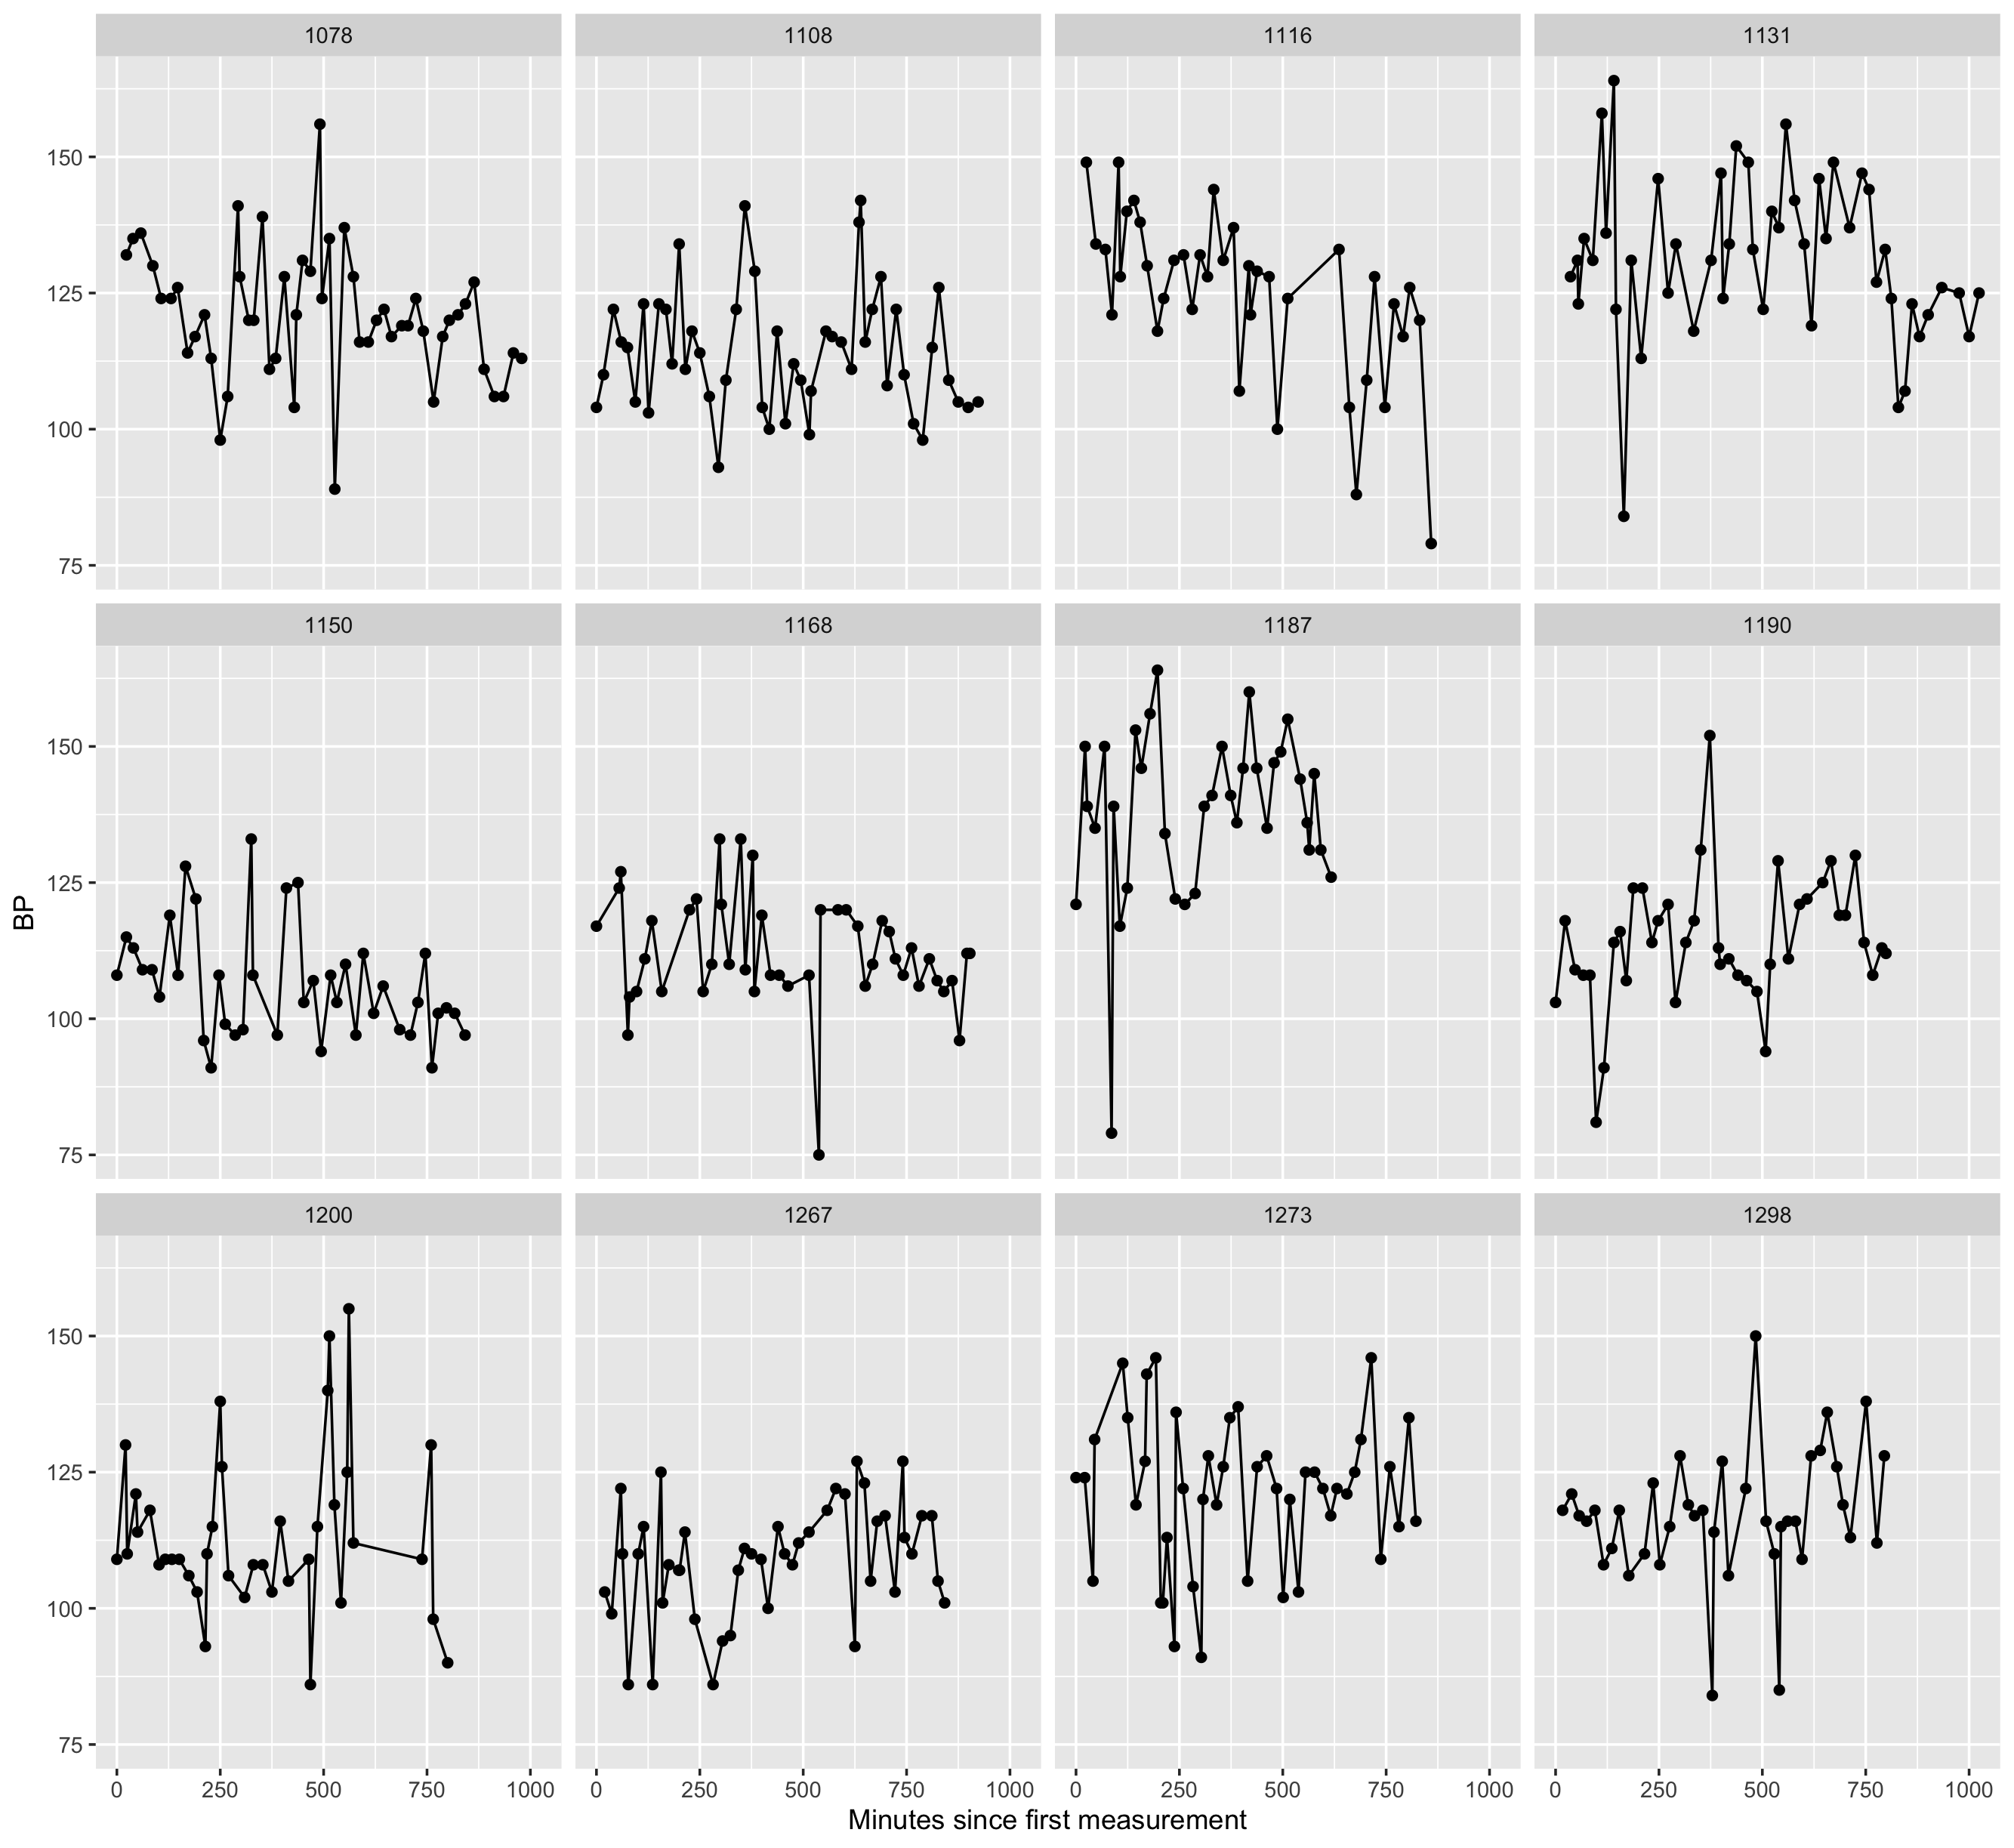
\includegraphics[width=\textwidth]{pics/bp v time by subj.png}
\caption[]%
{{\small BP vs. Time Passed by Subjects}}
\label{fig: bp v time facet}
\end{subfigure}
\hfill
\begin{subfigure}[b]{0.475\textwidth}
\centering
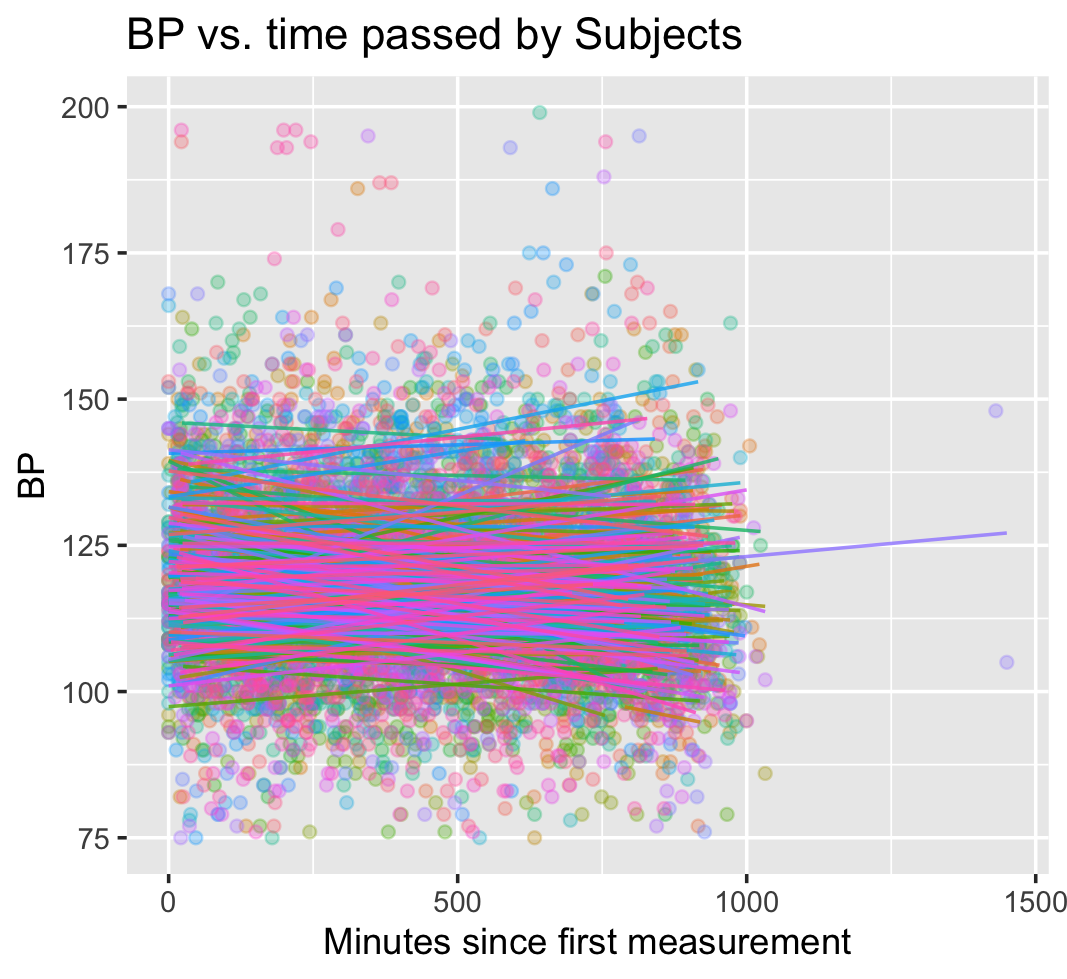
\includegraphics[width=\textwidth]{pics/BP v time LS.png}
\caption[]%
{{\small BP vs. Time Passed Separate Lines}}
\label{fig: bp v time separate ls}
\end{subfigure}
\caption[]
{\small BP vs. Minutes since first measurement}
\label{fig: bp v time}
\end{figure}


\begin{figure}
    \centering
    \begin{subfigure}[b]{0.29\textwidth}
    \centering
    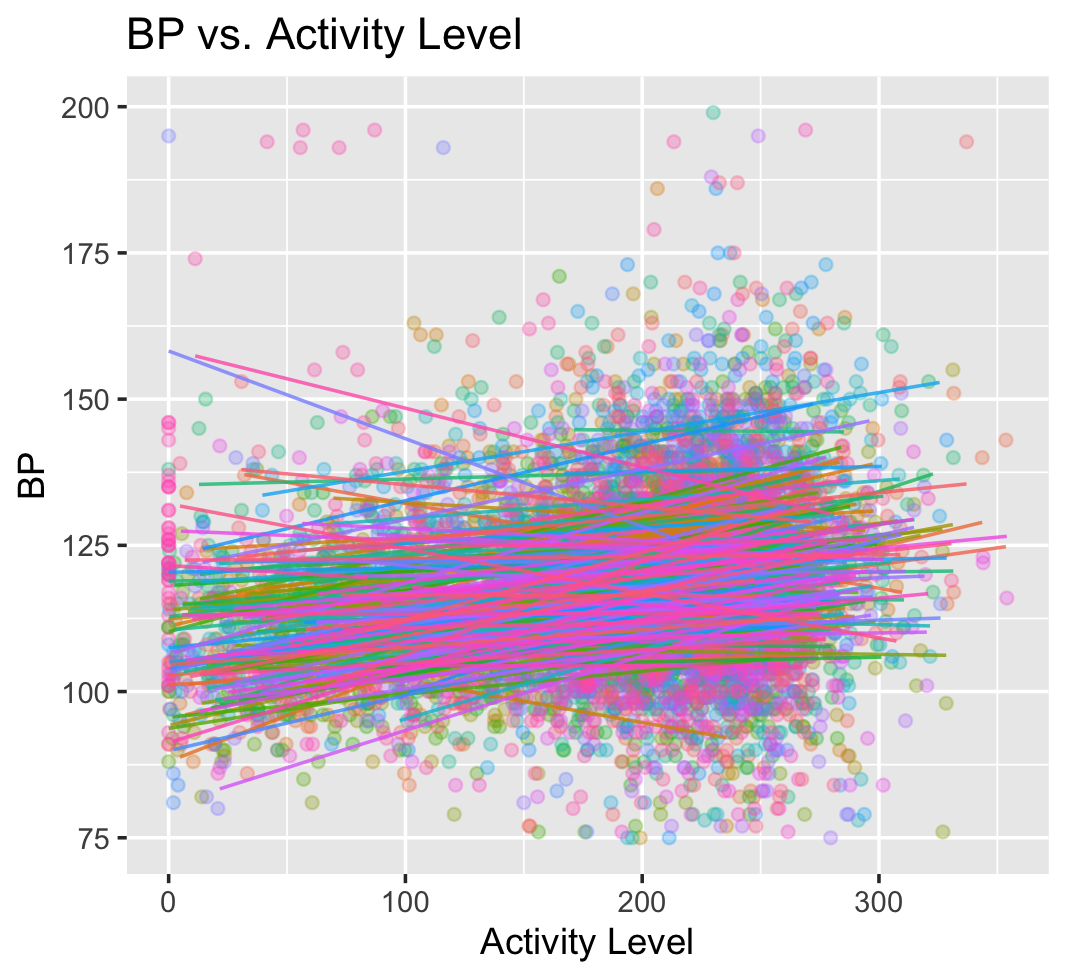
\includegraphics[width=\textwidth]{pics/bp v act.png}
    \caption[]%
    {{\small BP vs. Activity Level by Subjects}}
    \label{fig: bp v act}
    \end{subfigure}
    \hfill
    \begin{subfigure}[b]{0.29\textwidth}
    \centering
    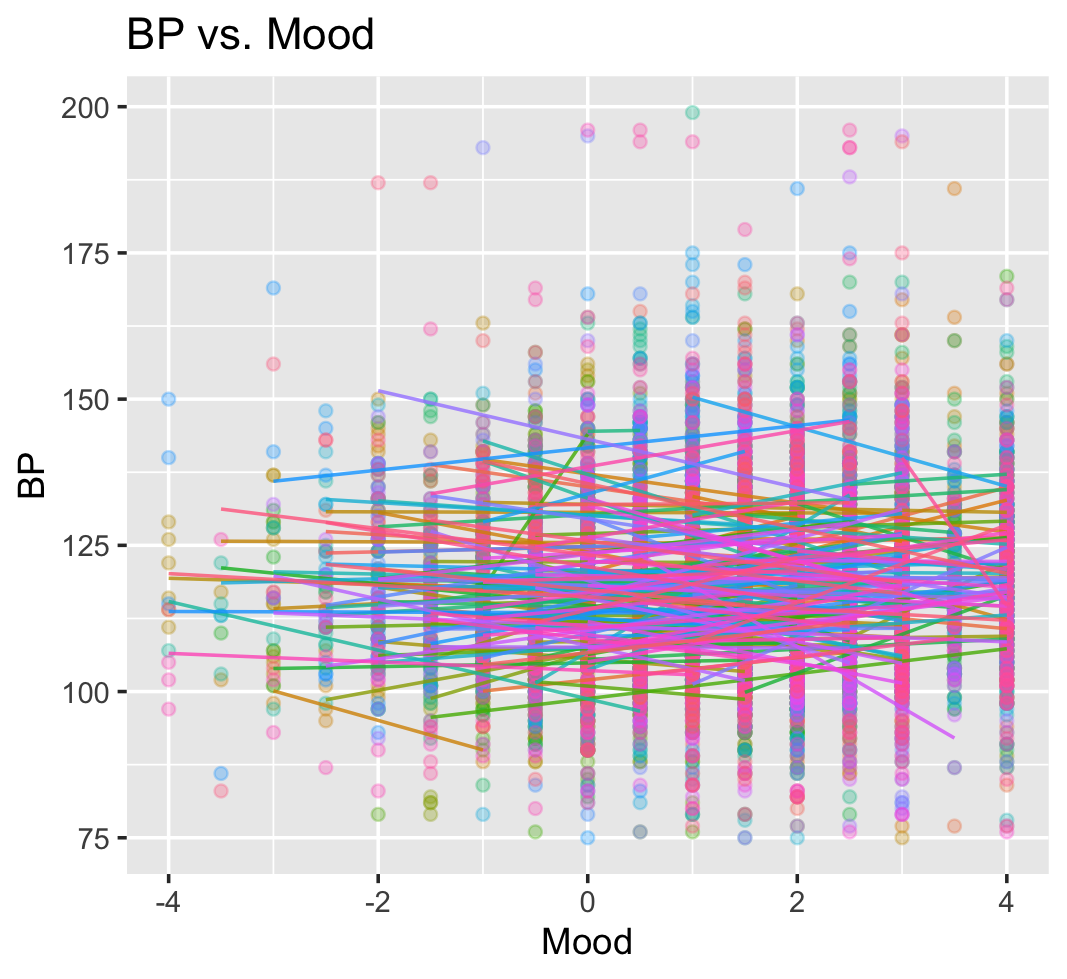
\includegraphics[width=\textwidth]{pics/bp v mood.png}
    \caption[]%
    {{\small BP vs. Mood by Subjects}}
    \label{fig: bp v mood}
    \end{subfigure}
    \hfill
    \begin{subfigure}[b]{0.29\textwidth}
    \centering
    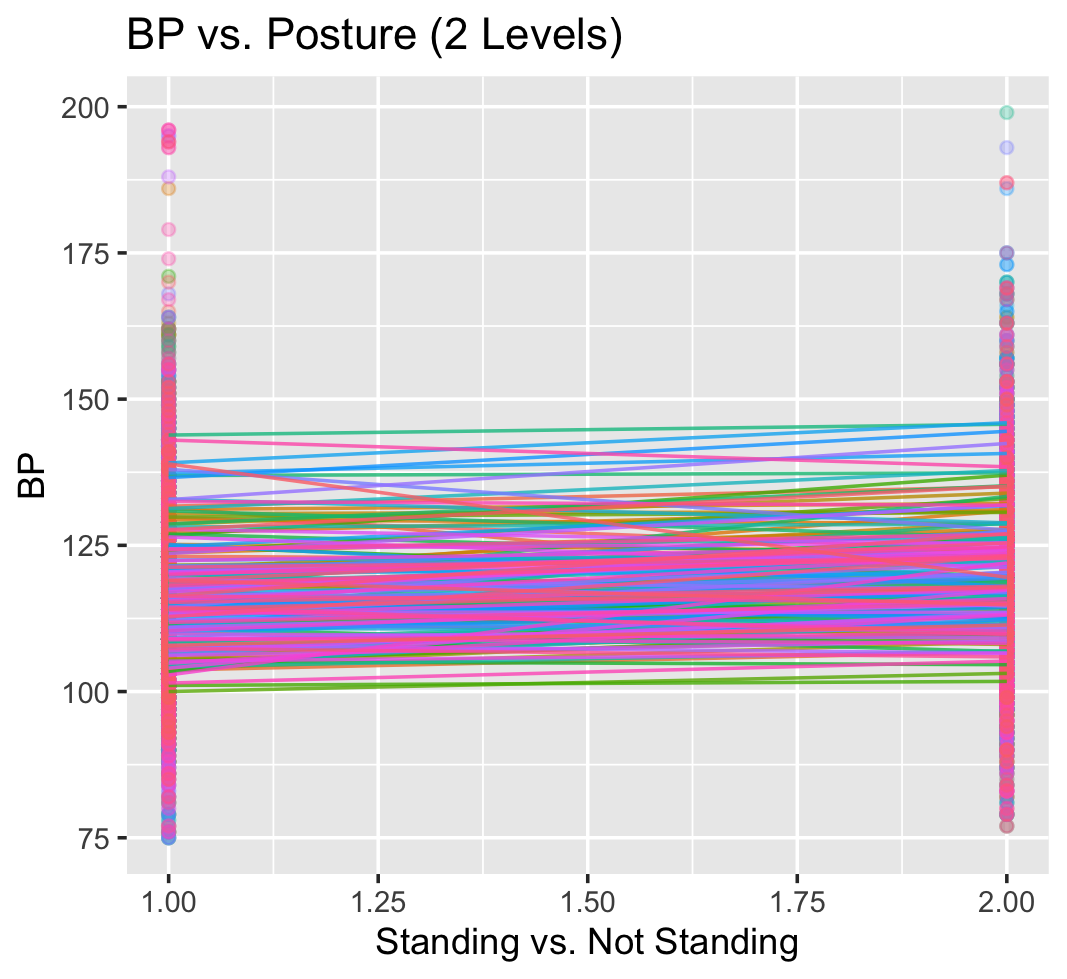
\includegraphics[width=\textwidth]{pics/bp v stand.png}
    \caption[]%
    {{\small BP vs. Posture by Subjects}}
    \label{fig: bp v stand}
    \end{subfigure}
    \caption[]
    {\small BP vs. Level 1}
    \label{fig: bp v level1}
    \end{figure}

We perform similar analysis for other level 1 covariates (see \Cref{fig: bp v level1}). We see the most prominent effect in \texttt{Mood}, where the slopes and intercepts for each participant differs the most. They all show, to a certain extend, signs of varying slopes and intercepts, but I cannot definitely conclude anything at this point.

\subsection{Level 2 Covariates}

We then want to understand the distributions of our level two covairates before we look at any interactions between the two levels. Because our level 2 covariates contains the same measurement over time (whereas our primary response \texttt{BP} is level 1 and hence time-dependent), we will compare the level 2 covariates with the \emph{average} \texttt{BP} of a given participant.



\begin{figure}
\centering
\begin{subfigure}[b]{0.475\textwidth}
\centering
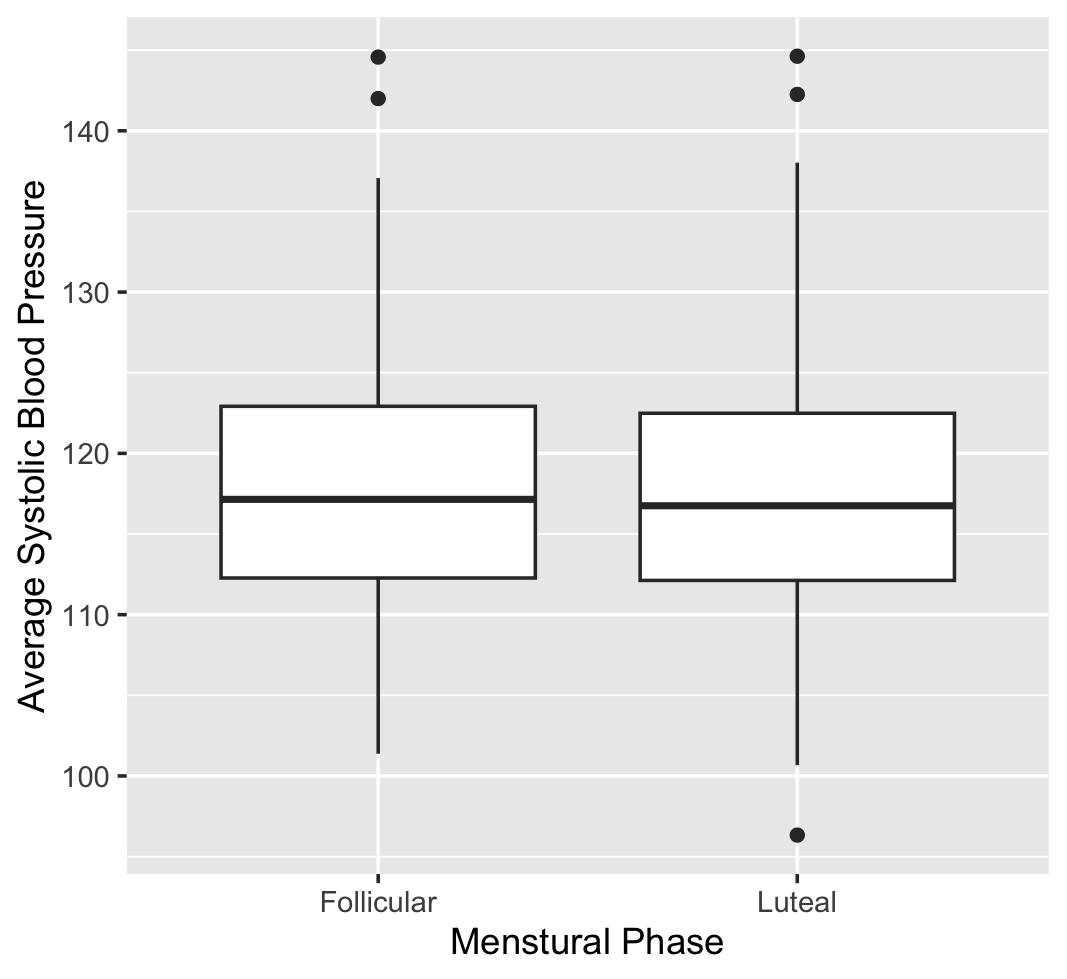
\includegraphics[width=\textwidth]{pics/bp v phase.png}
\caption[]%
{{\small Avg BP vs. Menstrual Phase}}
\label{fig: bp v phase}
\end{subfigure}
\hfill
\begin{subfigure}[b]{0.475\textwidth}
\centering
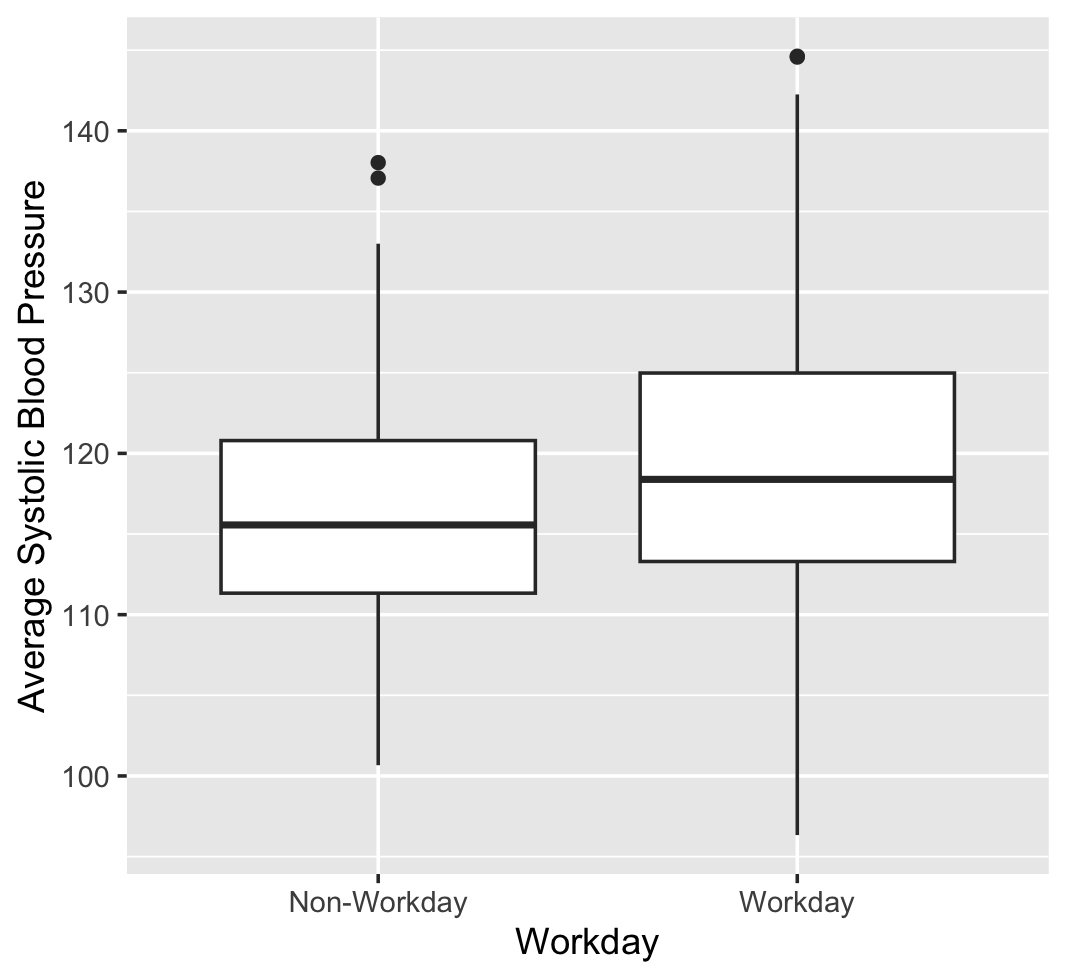
\includegraphics[width=\textwidth]{pics/bp v day.png}
\caption[]%
{{\small Avg BP vs. Workday}}
\label{fig: bp v day}
\end{subfigure}
\vskip\baselineskip
\begin{subfigure}[b]{0.475\textwidth}
    \centering
    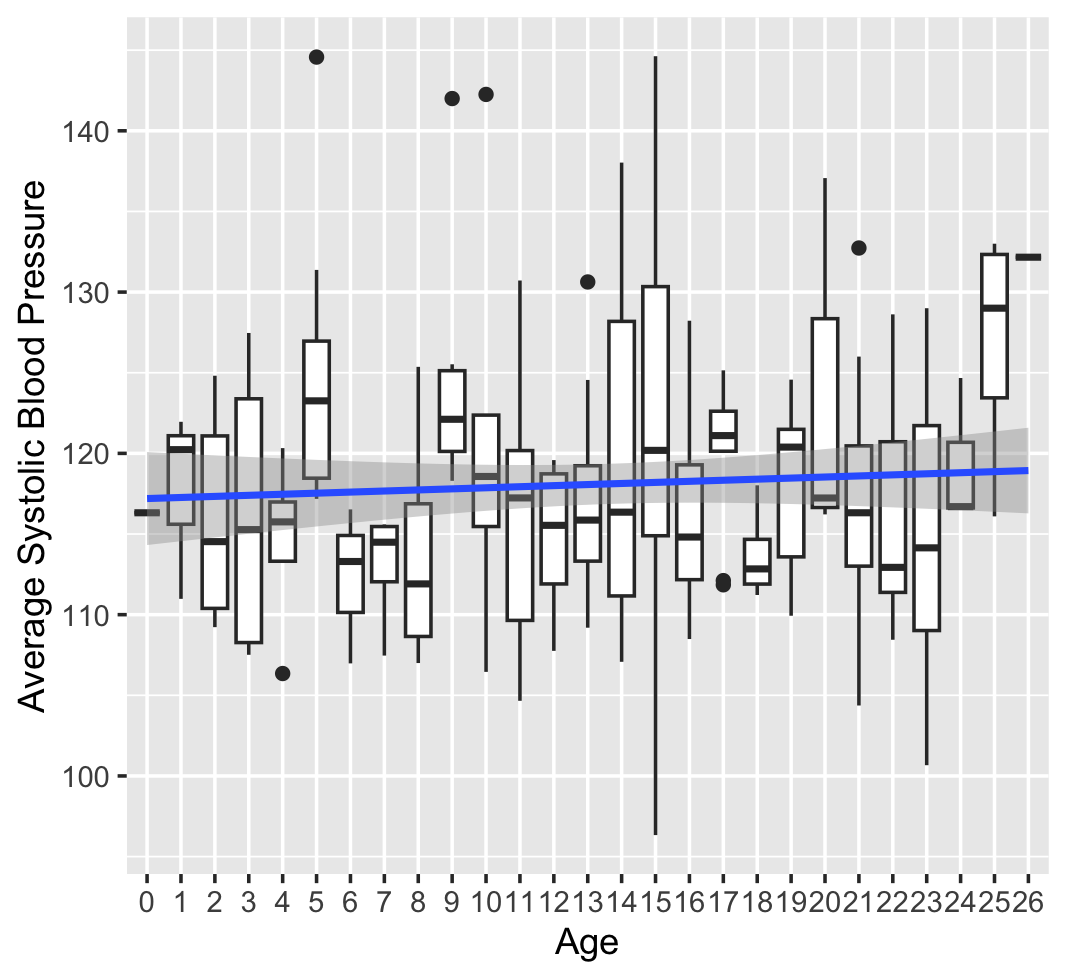
\includegraphics[width=\textwidth]{pics/bp v age.png}
    \caption[]%
    {{\small Avg BP vs. Age}}
    \label{fig: }
    \end{subfigure}
    \hfill
    \begin{subfigure}[b]{0.475\textwidth}
    \centering
    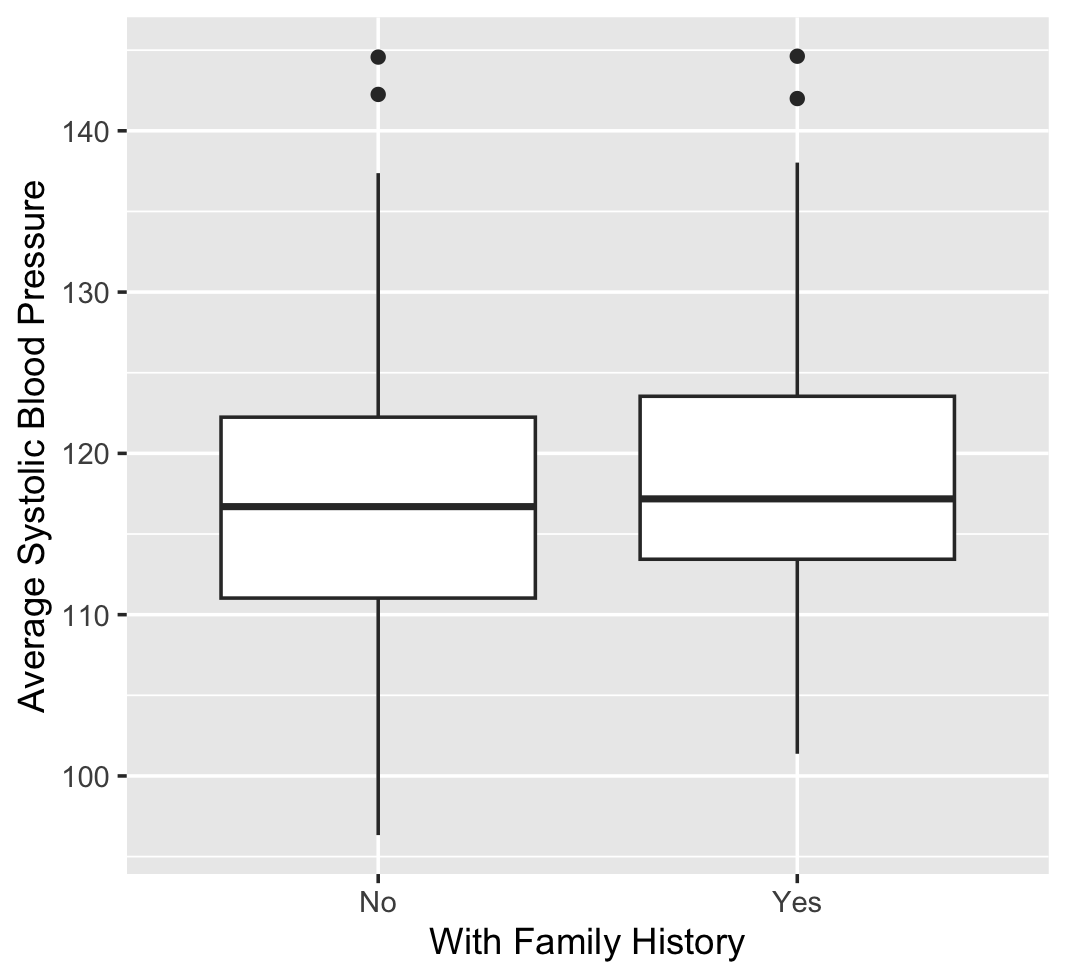
\includegraphics[width=\textwidth]{pics/bp v fh.png}
    \caption[]%
    {{\small }}
    \label{fig: }
    \end{subfigure}
\caption[]
{\small Average BP vs. Level 2 Covariates}
\label{fig: bp v level2}
\end{figure}

\subsection{Level 1 by Level 2 Covariates}

Next we investigate whether our level 1 covariates depend, in any way, on our level 2 covariates. 

\section{Model Selection}


\section{Results}

% \pagebreak
\singlespacing
% \bibliography{sources.bib}
% \bibliographystyle{apalike}
\printbibliography
% \detailtexcount{ccpaper}
\end{document}